\documentclass[9pt]{beamer}
\setbeamertemplate{navigation symbols}{}
\usepackage{minted}
\usepackage{algorithm2e}
\usepackage{multicol}
\usepackage{graphicx}
\usepackage{amsmath}
\usepackage{amssymb}
% \usepackage{subcaption}

\usepackage{caption}
\setminted{fontsize=\footnotesize}
\usemintedstyle{algol}
\usepackage{beamerthemeshadow}
\usepackage{tikz}
\usepackage{tikz-3dplot}
\usepackage{tikz}
\usetikzlibrary{tikzmark,calc}
\usepackage{csvsimple}

\setlength\columnsep{30pt}

\begin{document}
\title{JPEG2000 -- Wavelets and Compression}  
\author{Ben Keene}
\date{\today} 

\begin{frame}
	\titlepage
\end{frame}

\begin{frame}
	\begin{figure}[h]
		\centering
		\includegraphics[width=\textwidth]{./images/standards_2x.png}
		\tiny{Standards. xkcd. https://xkcd.com/927/ }
	\end{figure}	
\end{frame}

\section{Introduction}

\subsection{Image Formats}

\begin{frame}{Four Different Formats}
	\begin{multicols*}{2}
		\textbf{GIF}

		Developed in 1987 by CompuServe to
		distributed color images over slow modems.
		Allowed multiple images in a stream.
		Largely replaced by mp4.
		Uses LZW, a dictionary based lossless 
		compression algorithm.

		\vspace{1cm}

		\textbf{JPEG}

		Developed in 1992 by the
		Joint Photographic Experts Group.
		Designed for lossy compression via the
		Discrete Cosine Transform (DCT).
		Lossless JPEG introduced in 1993.

		% now do second column
		\columnbreak

		\textbf{PNG}

		Developed in 1996 to replace GIF,
		which required developers to pay royalties.
		PNG colloquially stands for "PNG's Not GIF".
		Uses a combination of pointers and encodings
		to achieve lossless compression.

		\vspace{1cm}

		\textbf{JPEG2000}

		Developed in 2000 to replace JPEG.
		Uses the Discrete Wavelet Transform (DWT)
		instead of DCT. Supports both lossless and
		lossy compression. Lossless compression 
		uses the Daubechies 5/3 wavelet, while lossy
		uses the Daubechies 9/7 wavelet.
		
	\end{multicols*}

\end{frame}

\section{The Discrete Wavelet Transform}

\subsection{1D}
\begin{frame}{1D DWT}
	Given a signal $(f_0, f_1, \dots, f_{n-1})$, where $n=2^J$, $(J \in \mathbb{N})$,
	then the function $f$ can be represented in a wavelet basis with coefficients $C_{00}$ and $d_{jk}$ as follows:
	\begin{equation*}
		f(x) = C_{00}\phi(x) + \sum_{j=0}^{J-1} \sum_{k=0}^{2^j-1} d_{jk} 2^{j/2} \psi(2^jx - k)
	\end{equation*}
	where
	\begin{itemize}
		\item[] $\phi$ is the scaling function (Father wavelet).
		\item[] $\psi$ is the wavelet function (Mother wavelet).
		\item[] $C_{00}$ is the scaling coefficient (average value of the signal).
		\item[] $d_{jk}$ are the wavelet coefficients of level $j$ at position $k$.
	\end{itemize}
\end{frame}



\begin{frame}{1D DWT}
	\begin{equation*}
		f(x) = \underbrace{\tikzmarknode{c00}{{C_{00}}}\phi(x)}_{(1)} +
		\underbrace{\sum_{j=0}^{J-1}
		\sum_{k=0}^{2^j-1}}_{(3)}
		\tikzmarknode{djk}{d_{jk}}
		\underbrace{2^{j/2} \psi(2^jx - k)}_{(2)}
	\end{equation*}
	\begin{tikzpicture}[overlay,remember picture]
		\draw[<-, black] (djk) -- ++(0.2,-1.5) node[below] {
			$\frac{
				\langle f, \psi_{j,k} \rangle
			}
			{||\psi_{j,k}||^2}$

		};
		\draw[<-, black] (c00) -- ++(-0.5,-1) node[below] {
			$\frac{
				\langle f, \phi_{0,0} \rangle
			}
			{||\phi_{0,0}||^2}$
		};
	\end{tikzpicture}
	\vspace{1cm}
	\begin{itemize}
		\item[] (1) represents the coarsest approximation of $f$. What does $f$ look like from the perspective of the scaling function?
		\item[] (2) is the tool with which we are measuring $f$ at a very fine resolution.
		\item[] (3) ensures we are measuring $f$ over all positions $k$ and resolutions $j$.
	\end{itemize}
\end{frame}
\subsection{Colors and Wavelets}
\begin{frame}{Color space}
A color space is a way of representing colors as tuples of numbers.
Some examples are RGB (red, green, blue), CMY (cyan, magenta, yellow), HSL (hue, saturation, lightness), and HSV (hue, saturation, value).

\vspace{1cm}

JPEG2000 relies upon YCbCr (luminance, blue chrominance, red chrominance) for ossy compression.

\vspace{1cm}

There doesn't exist a bijection between the two color spaces, but since YCbCr offers 
better compression, images are converted before the DWT.

\vspace{1cm}

Lossless compression, outside the scope of this presentation, uses the YUV color space.

\end{frame}

\begin{frame}{CDF 9-tap/7-tap wavelet}

The Cohen-Daubechies-Feauveau (CDF) 9-tap/7-tap wavelet (also called the Biorthogonal 4.4 wavelet)
is used for lossy compression in JPEG2000.

\begin{itemize}
	\item[] CDF $M$-tap/$N$-tap wavelets are wavelets with $M$ coefficients for the decomposition scaling function and $N$ coefficients for the reconstruction scaling function.
	\item[] Biorthogonal $M$.$N$ wavelets have $M$ vanishing moments in the reconstruction wavelet and $N$ vanishing moments in the decomposition wavelet.
\end{itemize}

\begin{figure}
    \centering
	\small
    \begin{tabular}{|r|r|r|r|r|}\hline%
    $k$ & $\text{dec}_\text{lo}$ & $\text{dec}_\text{hi}$ & $\text{rec}_\text{lo}$ & $\text{rec}_\text{hi}$ \\\hline\hline
    \csvreader[
        late after line = \\\hline,
        ]{./tables/cdf97.csv}%
        {k=\k, declo=\declo, dechi=\dechi, reclo=\reclo, rechi=\rechi}%
        {\k & \declo & \dechi & \reclo & \rechi}%
    \end{tabular}
\end{figure}
	
\end{frame}

\begin{frame}{CDF 9/7 Plots}
	\begin{figure}[h]
		\centering
		\includegraphics[width=\textwidth]{./plots/cdf97.png}
		\caption{Scaling and Wavelet functions for CDF 9/7}
	\end{figure}
\end{frame}
\begin{frame}{Approximation}
		\begin{equation*}
			\text{Consider:     }f(x) = \sin\left(\frac x {16}\right) + \sin\left(\frac x {32}\right) + \sin\left(\frac x {64}\right)
		\end{equation*}
		The approximation of $f$ via the DWT with CDF 9/7 wavelet is not too bad.
		\begin{figure}[h]
			\centering
			\includegraphics[scale=0.5]{./plots/cdf97_dwt.png}
		\end{figure}
\end{frame}

\begin{frame}{Reconstruction}
	As expected, we get perfect reconstruction.
	\begin{figure}[h]
		\centering
		\includegraphics[scale=0.5]{./plots/cdf97_idwt.png}
	\end{figure}
	
\end{frame}

\subsection{2D DWT}
\begin{frame}{2D DWT: Notation}
	\begin{itemize}
		\item[] $\Phi(x,y) = \phi(x)\phi(y)$: 2D scaling function.
		\item[] $\Psi^H(x,y) = \psi(x)\phi(y)$: Horizontal wavelet function.
		\item[] $\Psi^V(x,y) = \phi(x)\psi(y)$: Vertical wavelet function.
		\item[] $\Psi^D(x,y) = \psi(x)\psi(y)$: Diagonal wavelet function.
		\item[] $\Phi_{jmn}(x,y) = 2^{j/2} \Phi(2^jx-m, 2^jy-n)$: 2D scaling function at level $j$ and position $(m,n)$.
		\item[] $\Psi^\alpha_{jmn}(x,y) = 2^{j/2} \Psi^\alpha(2^jx-m, 2^jy-n)$: 2D wavelet function at level $j$ and position $(m,n)$ for orientation $\alpha \in \{H, V, D\}$.
	\end{itemize}
\end{frame}
\begin{frame}{2D DWT: Notation}
Given a 2D signal $f(x,y)$ of size $M \times N$, the 2D Discrete Wavelet Transform relates to $f$ via:

For simplicity, assume $M = N = 2^J$ for some $J \in \mathbb{N}$.
Then, we can construct a representation of $f$ in a wavelet basis as follows:


\begin{equation*}
f(x,y) = C_{000}\Phi(x,y)+ \sum_{\alpha \in {H, V, D}} \sum_{j=0}^{J-1} \sum_{m=0}^{2^j-1} \sum_{n=0}^{2^j-1} d^\alpha_{jmn} 2^{j/2} \Psi^\alpha(2^jx-m, 2^jy-n)
\end{equation*}
where
\begin{itemize}
\item[] $C_{000}$ is the 2D scaling coefficient (average value of the signal).
\item[] $d^\alpha_{jmn}$ are the wavelet coefficients for orientation $\alpha$ at level $j$ and position $(m,n)$.
\end{itemize}
\end{frame}



\begin{frame}{2D DWT}
	\begin{equation*}
        f(x,y) = \underbrace{\tikzmarknode{c000}{C_{000}}\Phi(x,y)}_{(1)} 
    	+ \underbrace{\sum_{\alpha \in {H, V, D}} \sum_{j=0}^{J-1} \sum_{m=0}^{2^j-1} \sum_{n=0}^{2^j-1}}_{(3)} \tikzmarknode{dalpha}{d^\alpha_{jmn}} \underbrace{2^{j/2} \Psi^\alpha(2^jx-m, 2^jy-n)}_{(2)}
	\end{equation*}
    \begin{tikzpicture}[overlay,remember picture]
        \draw[<-, black] (dalpha) -- ++(0.2,-1.5) node[below] {
            $\frac{
                \langle f, \Psi^\alpha_{j,m,n} \rangle
            }
            {||\Psi^\alpha_{j,m,n}||^2}$
        };
        \draw[<-, black] (c000) -- ++(-0.5,-1) node[below] {
            $\frac{
                \langle f, \Phi_{0,0,0} \rangle
            }
            {||\Phi_{0,0,0}||^2}$
        };
    \end{tikzpicture}
    \vspace{1cm}
    \begin{itemize}
        \item[] (1) represents the coarsest approximation of $f$. What does $f$ look like from the perspective of the scaling function?
        \item[] (2) is the tool with which we are measuring $f$ at a very fine resolution.
        \item[] (3) ensures we are measuring $f$ over all positions $(m,n)$ and resolutions $j$ for each orientation $\alpha$.
    \end{itemize}
\end{frame}

\section{Implementation}



\subsection{Decomposition}

\begin{frame}{Our Subject}
	\begin{figure}[h]
		\centering
		\includegraphics[scale=0.2]{./data/cat.jpg}
		\caption{Ava, \tiny short for Avocado}
	\end{figure}
	Next, let's split into RGB as a toy example.
\end{frame}

\begin{frame}{RGB}
	\begin{figure}[h]
		\centering
		\includegraphics[width=\textwidth]{./plots/channelsplit.png}
	\end{figure}
\end{frame}

\begin{frame}{Level 1}
	\begin{figure}
		\centering
		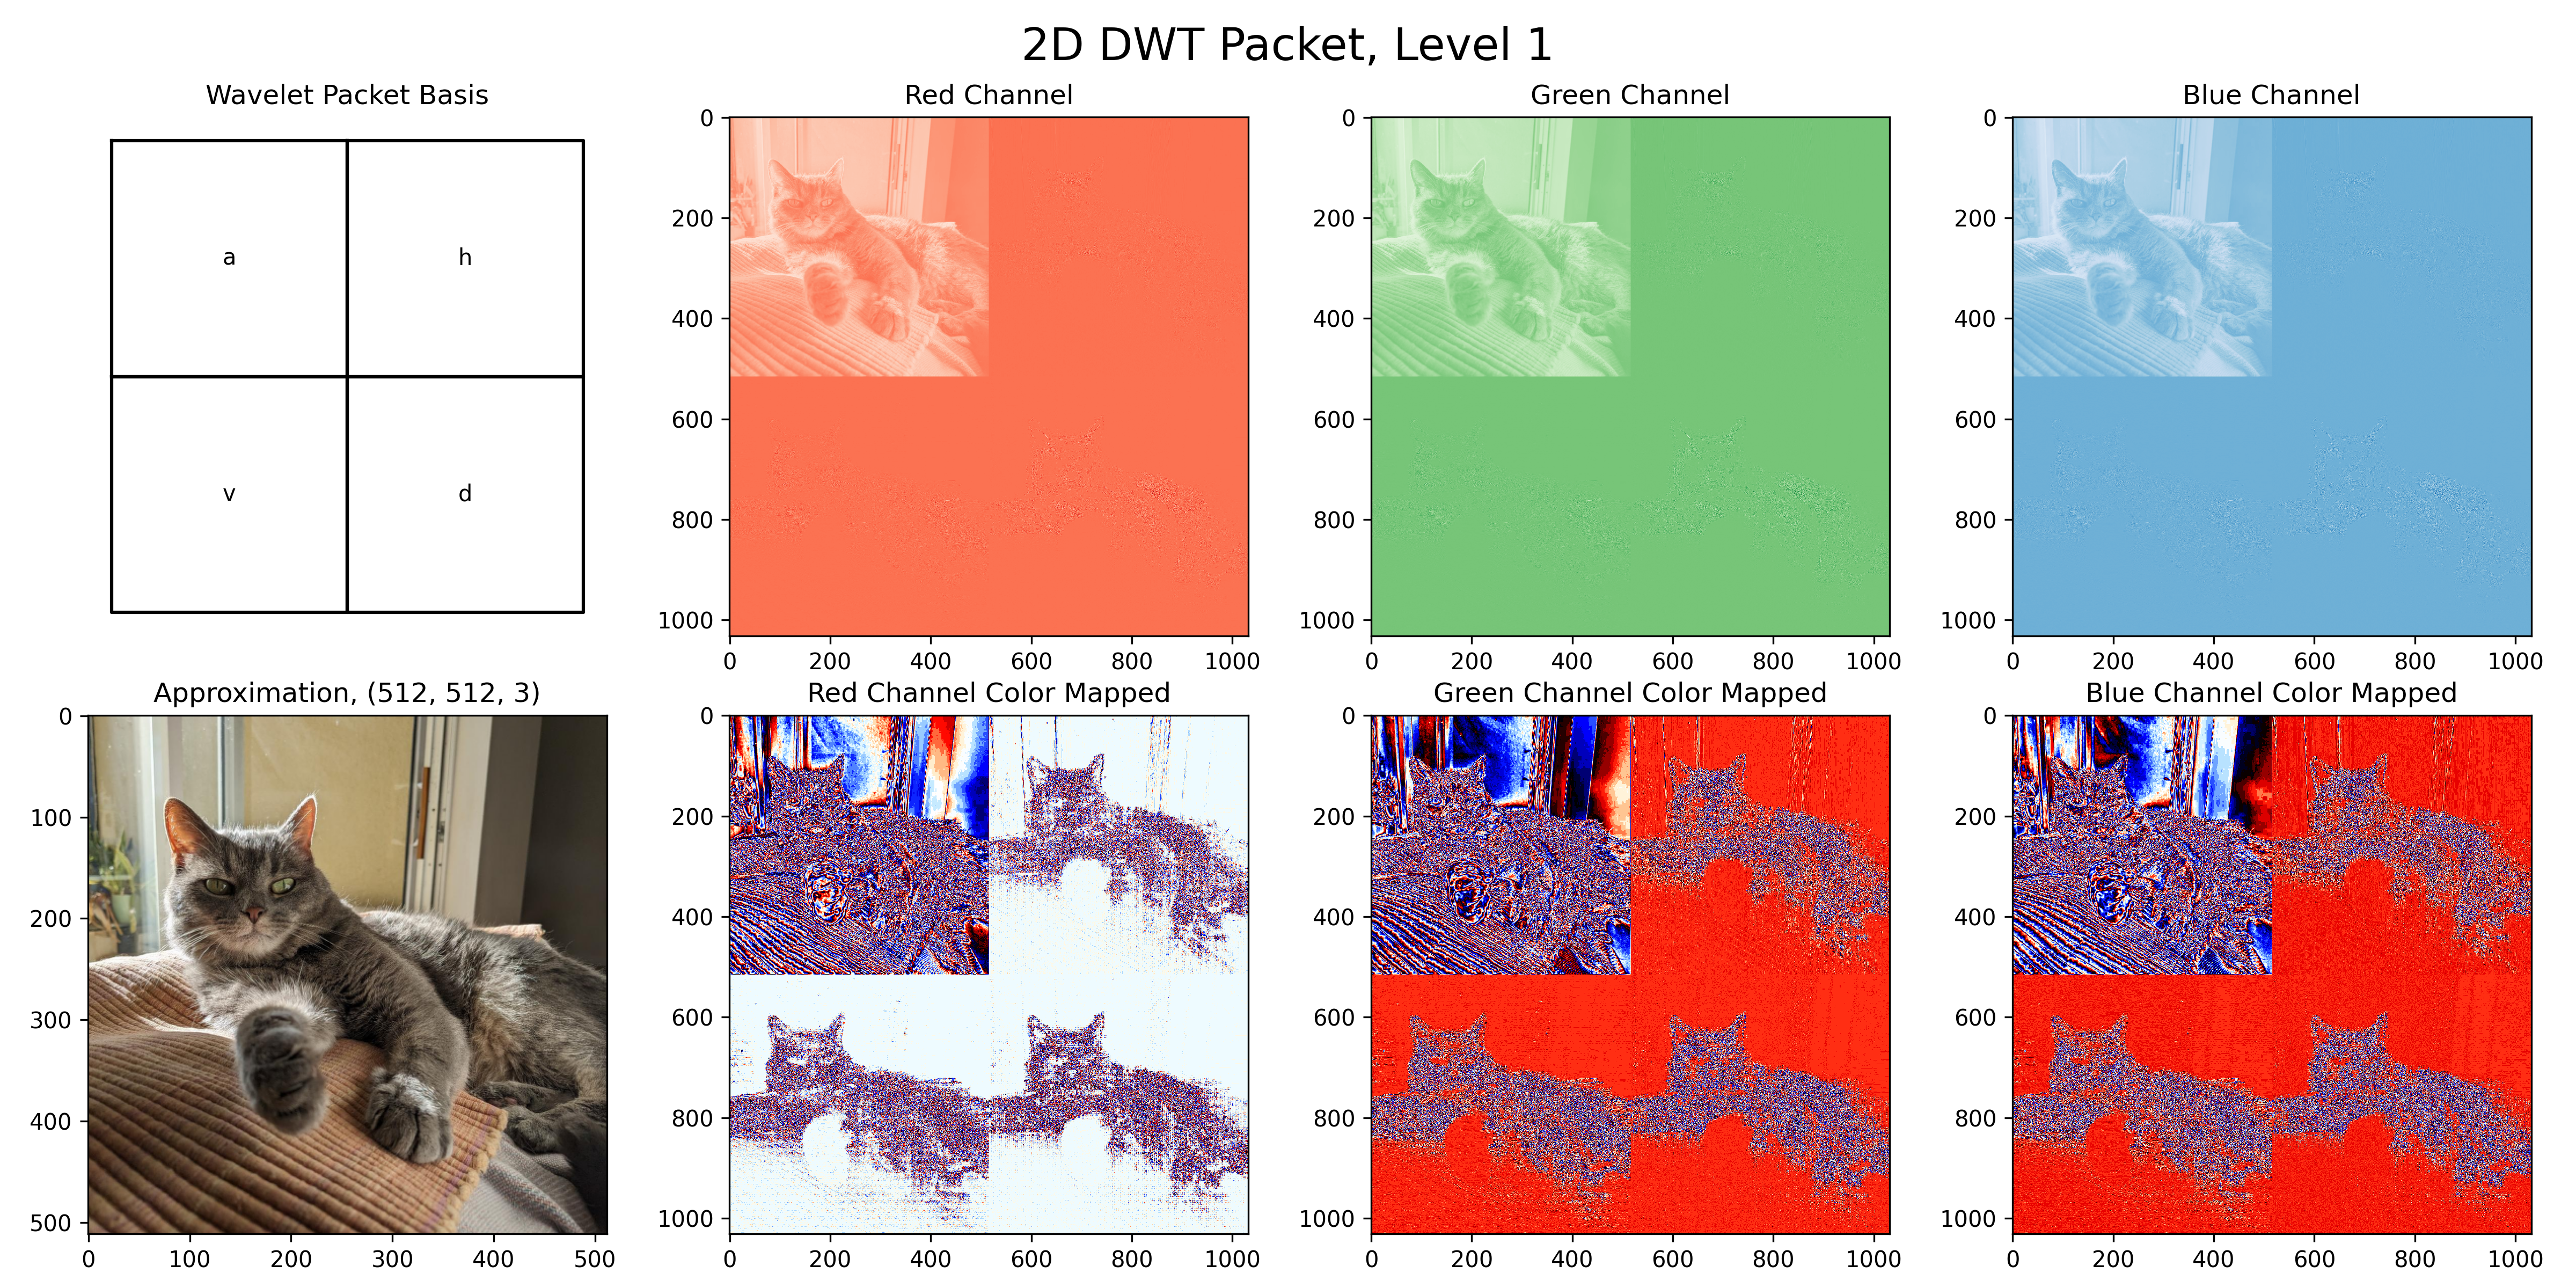
\includegraphics[scale=0.25]{./plots/level_1.png}
	\end{figure}
\end{frame}

\begin{frame}{Level 2}
	\begin{figure}
		\centering
		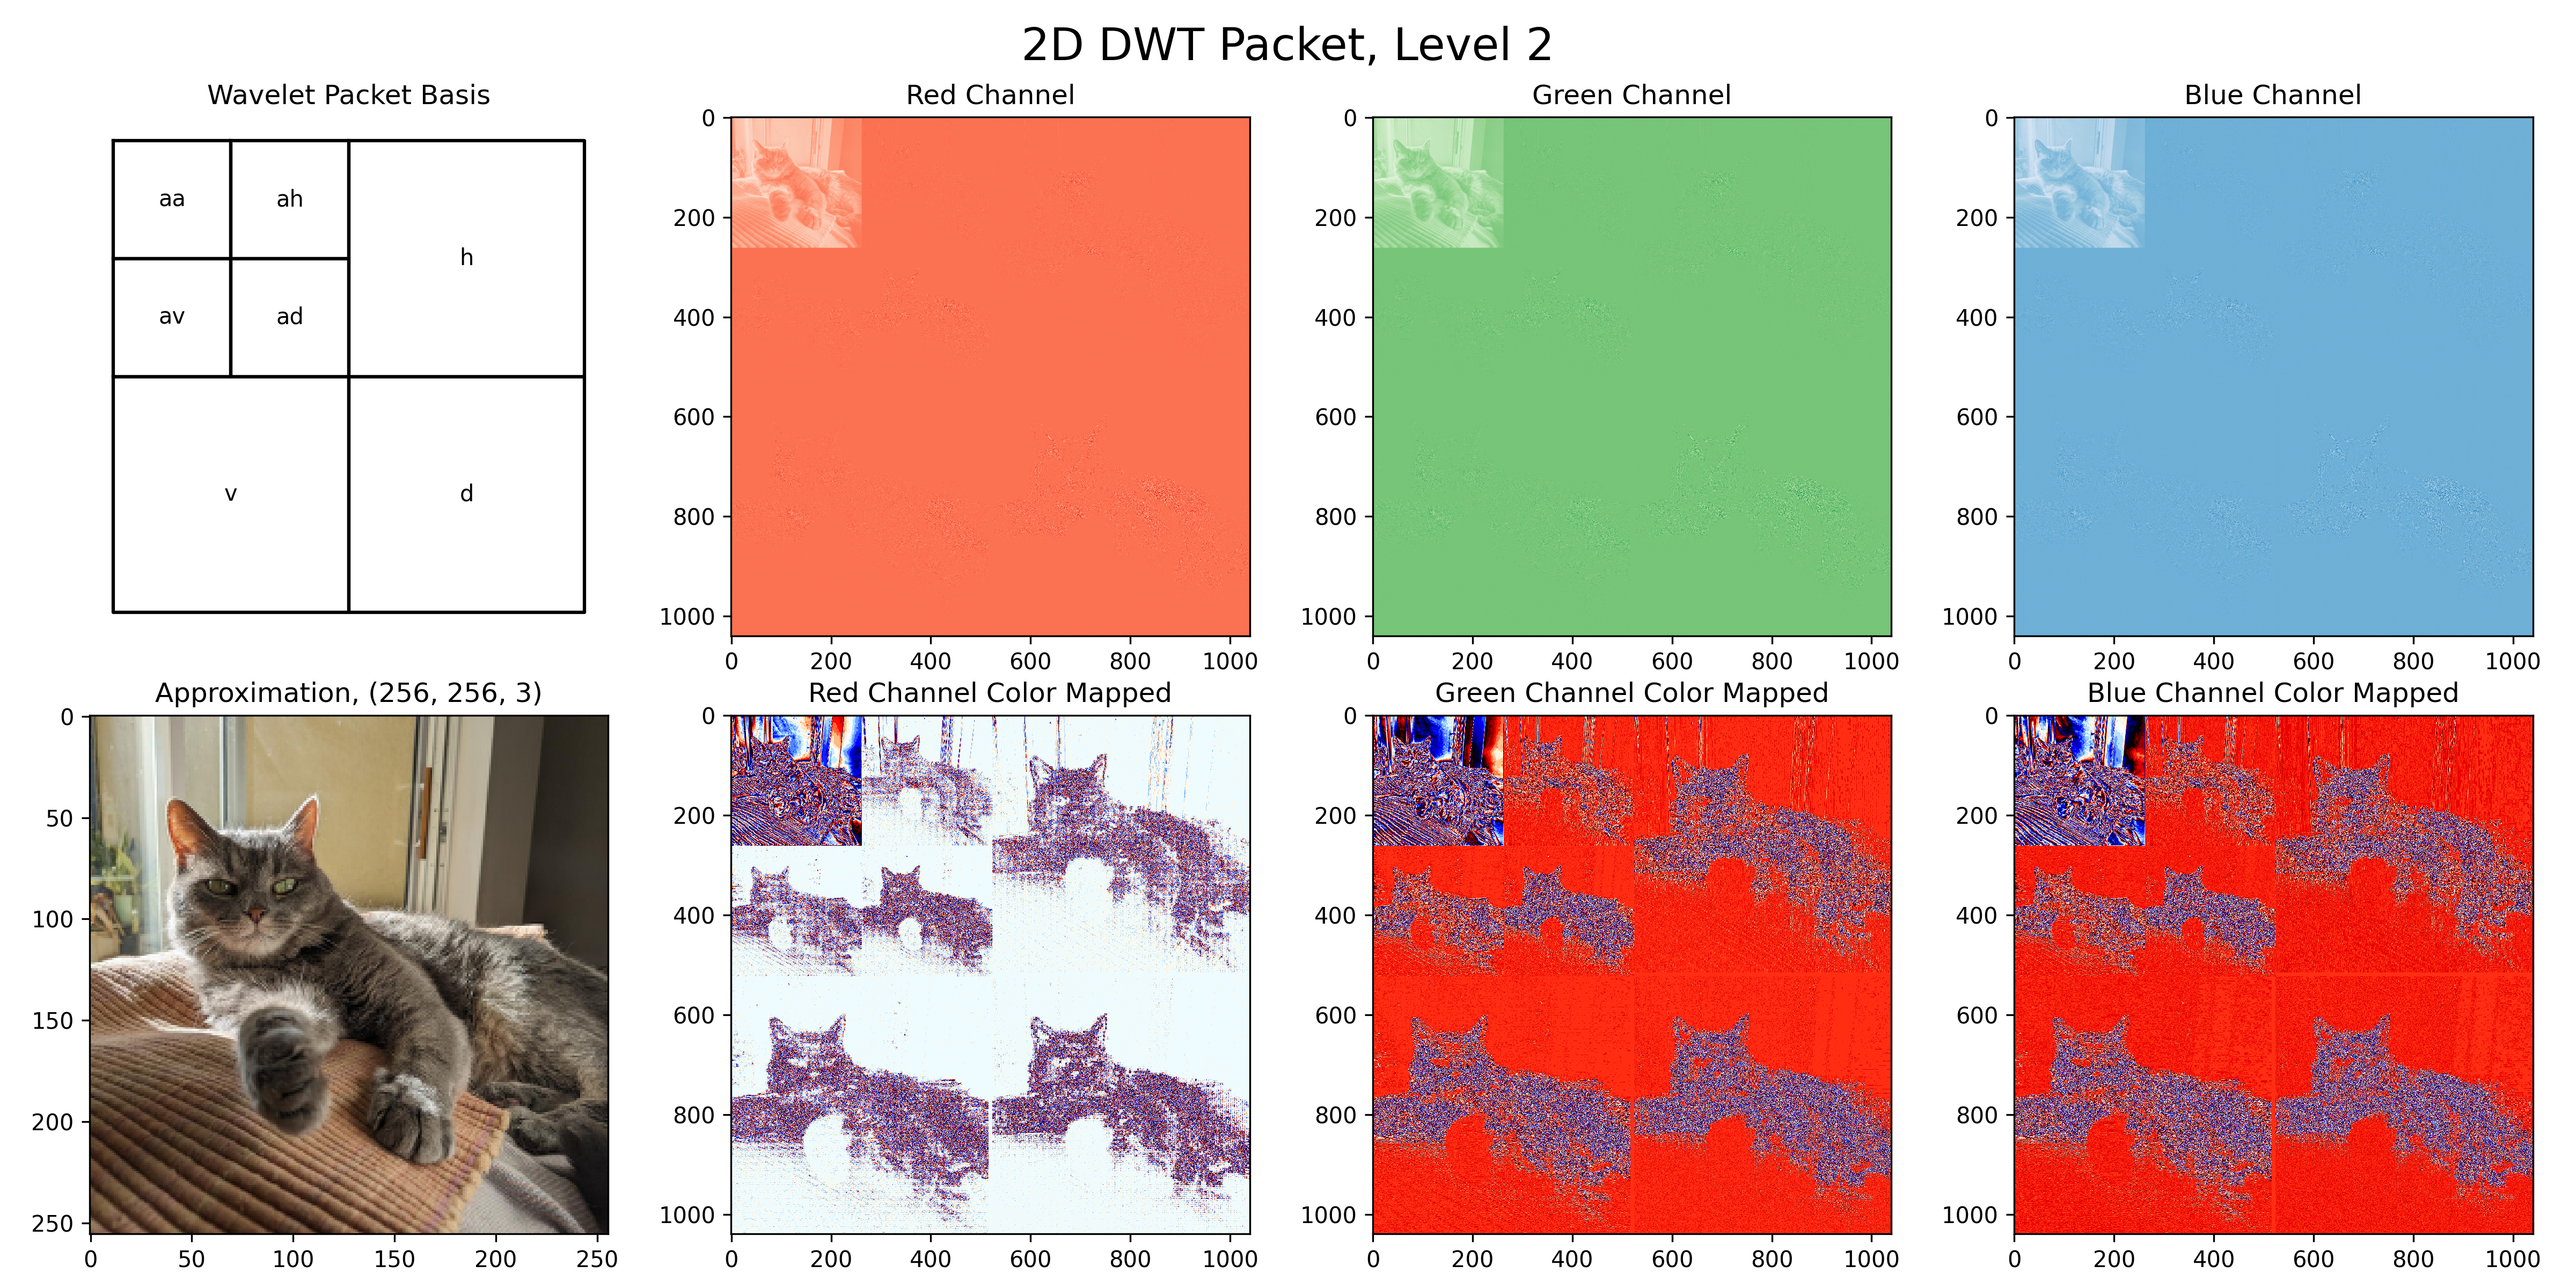
\includegraphics[scale=0.25]{./plots/level_2.png}
	\end{figure}	
\end{frame}

\begin{frame}{Level 3}
	\begin{figure}
		\centering
		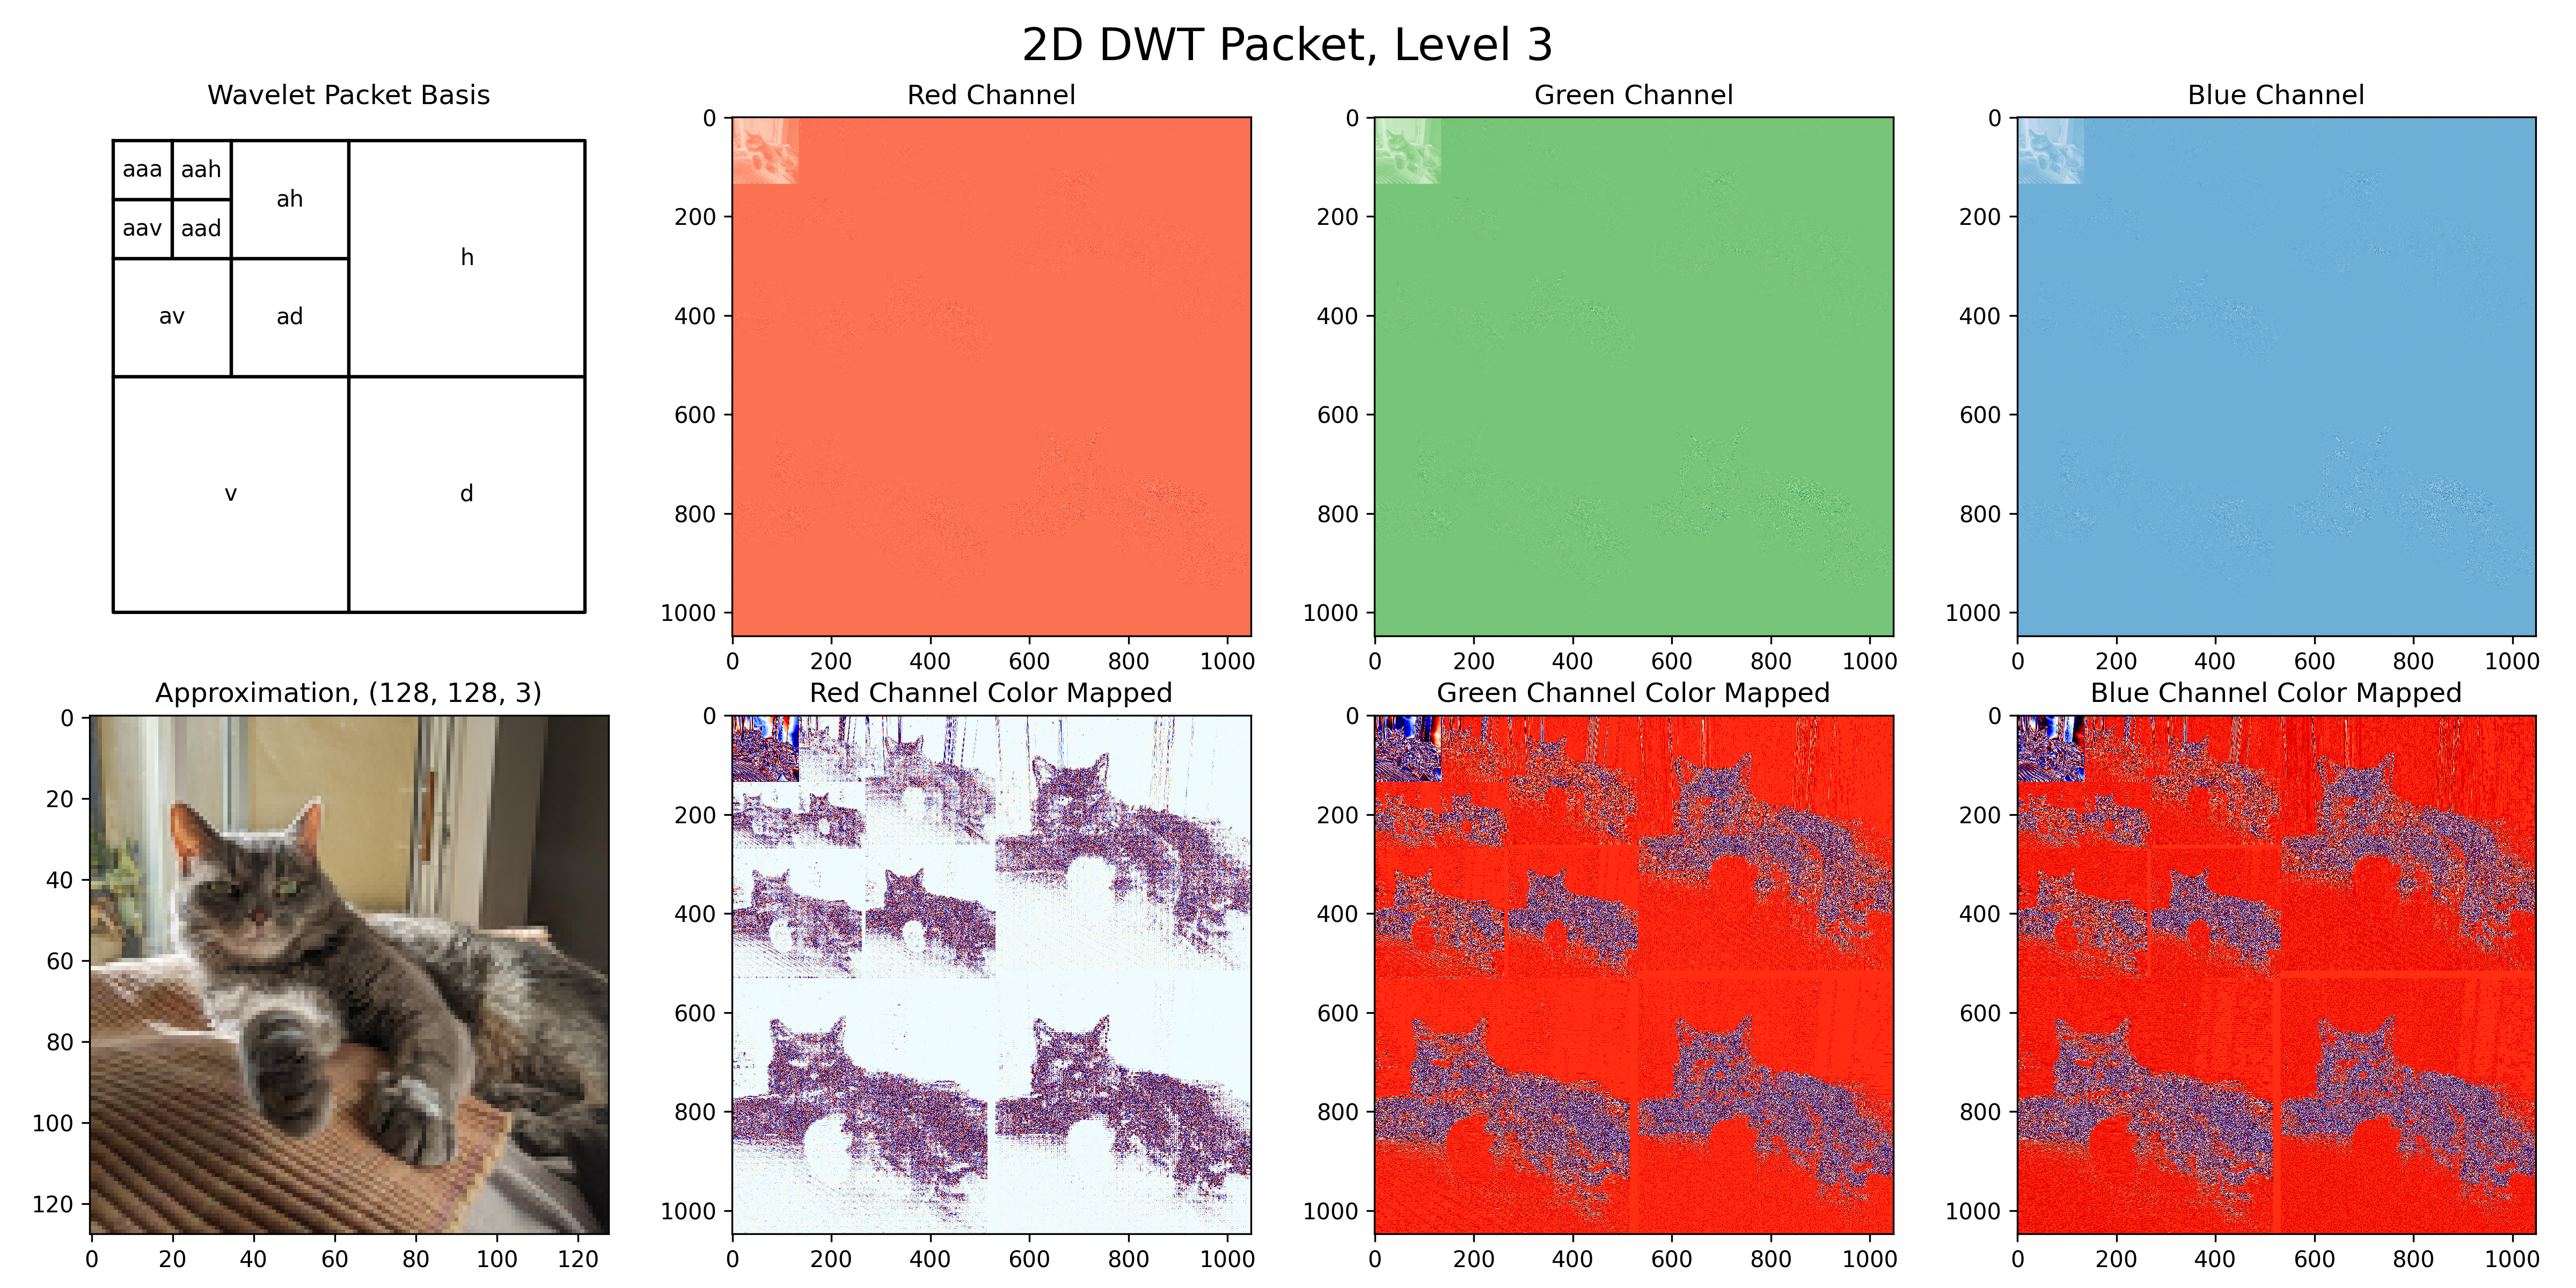
\includegraphics[scale=0.25]{./plots/level_3.png}
	\end{figure}
\end{frame}

\begin{frame}{Level 4}
	\begin{figure}
		\centering
		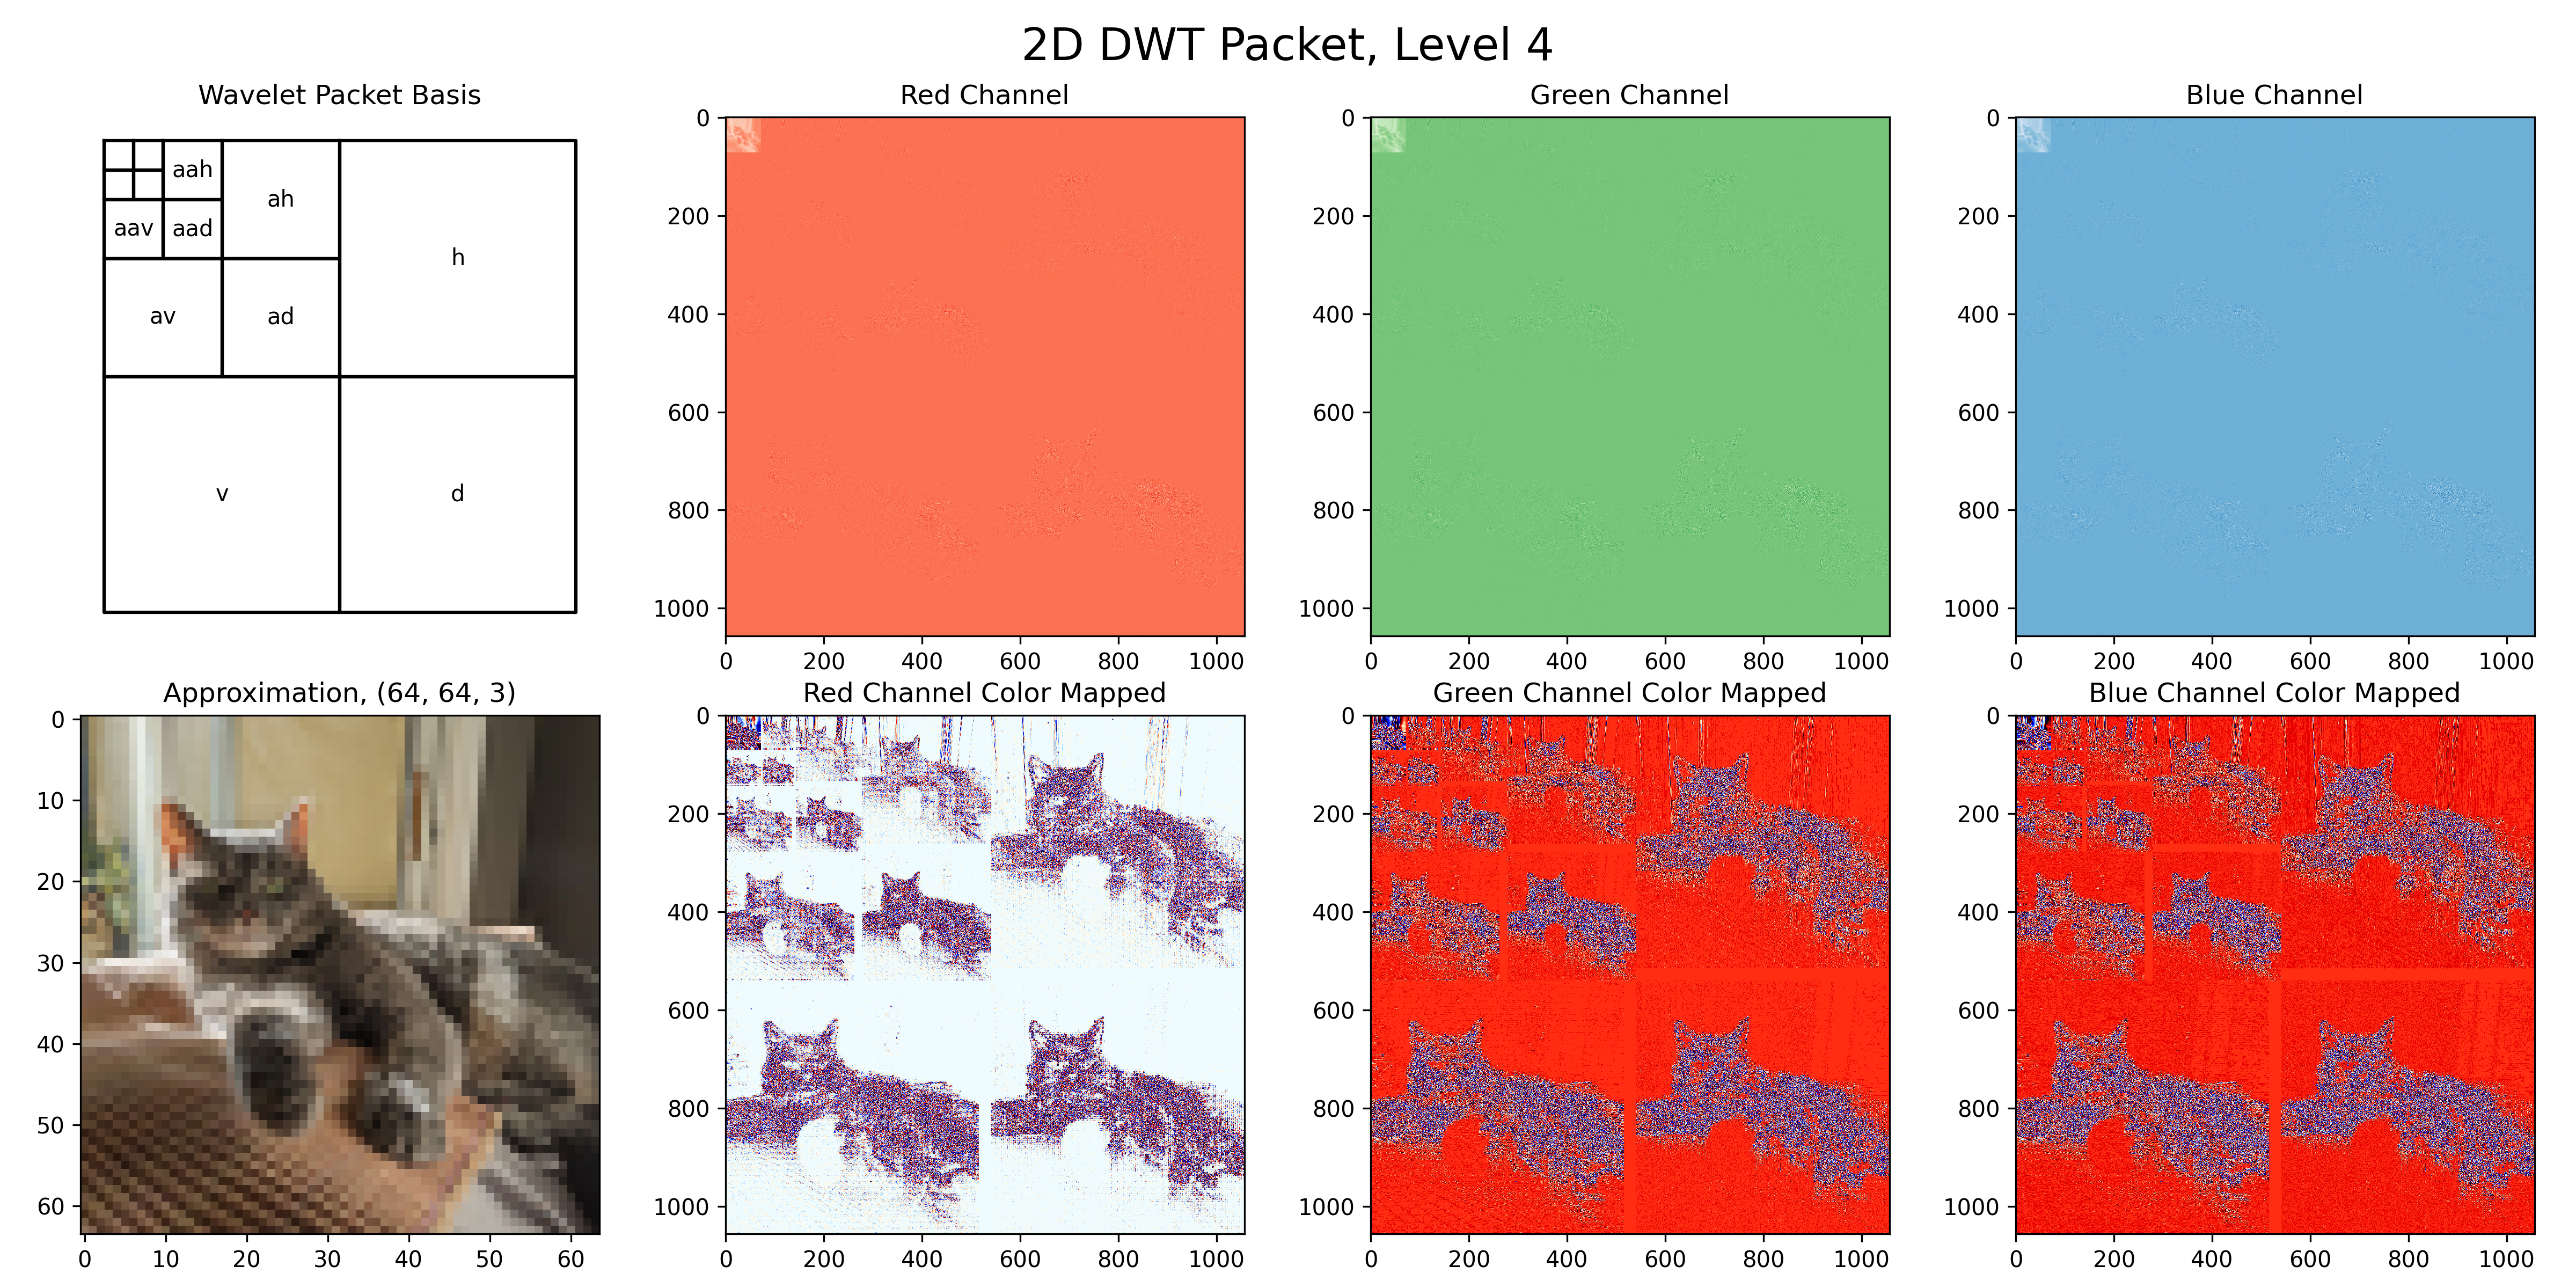
\includegraphics[scale=0.25]{./plots/level_4.png}
	\end{figure}
\end{frame}

\begin{frame}{Level 5}
	\begin{figure}
		\centering
		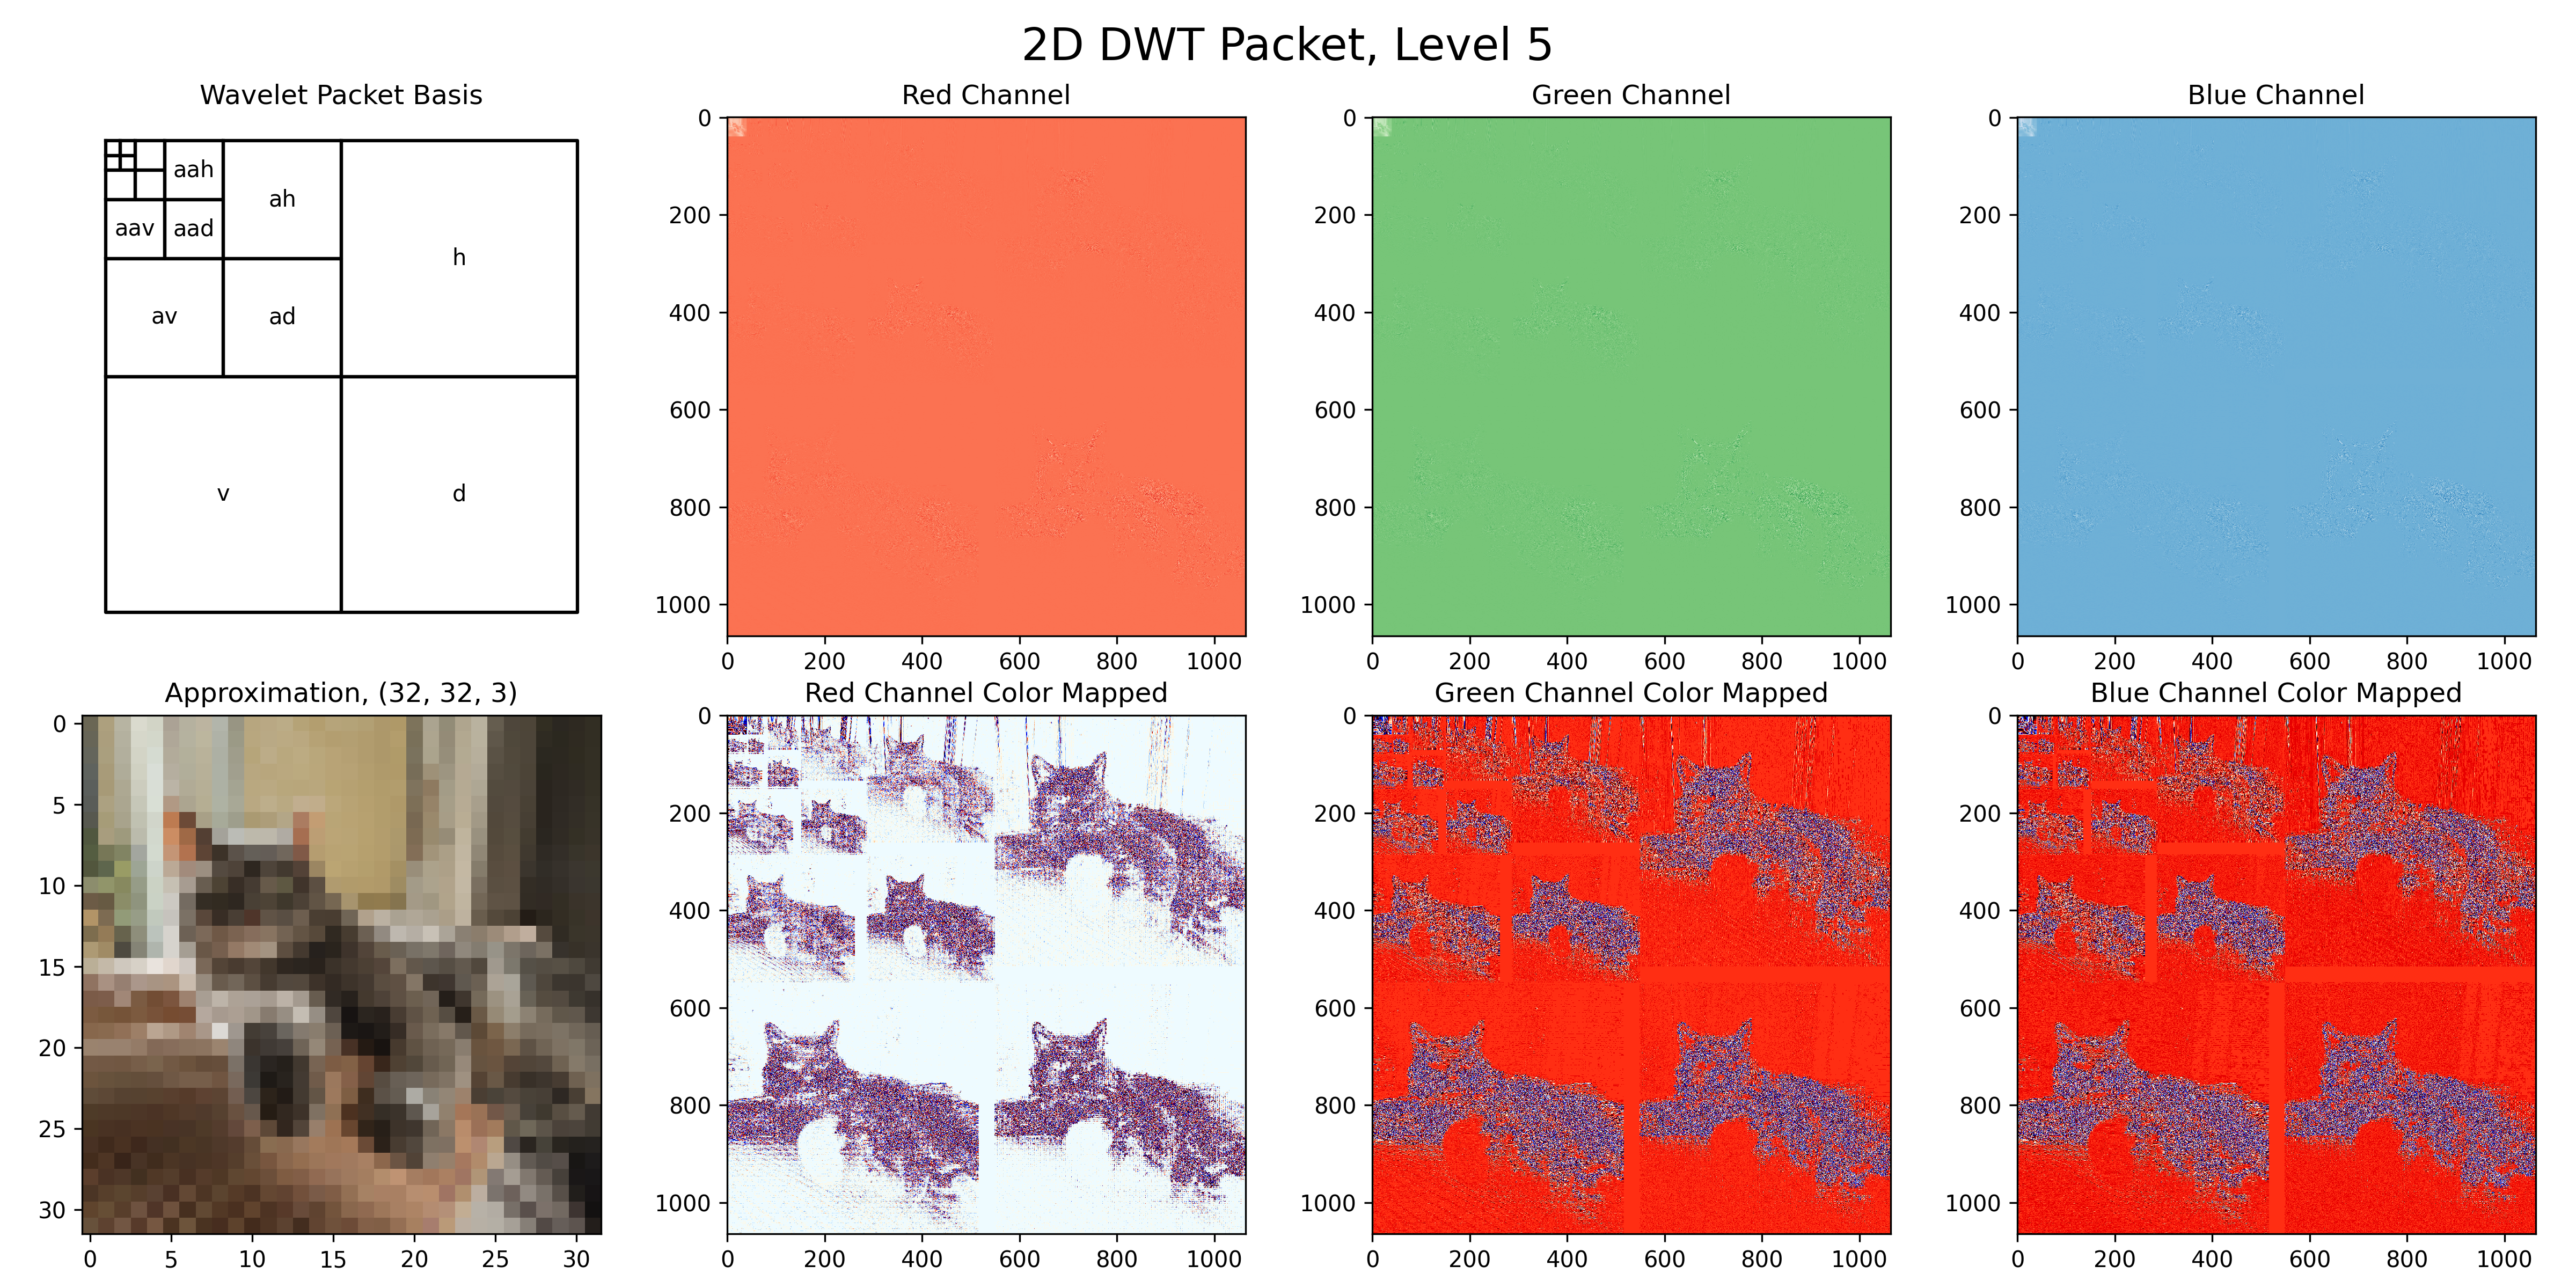
\includegraphics[scale=0.25]{./plots/level_5.png}
	\end{figure}
\end{frame}

\begin{frame}{Level 6}
	\begin{figure}
		\centering
		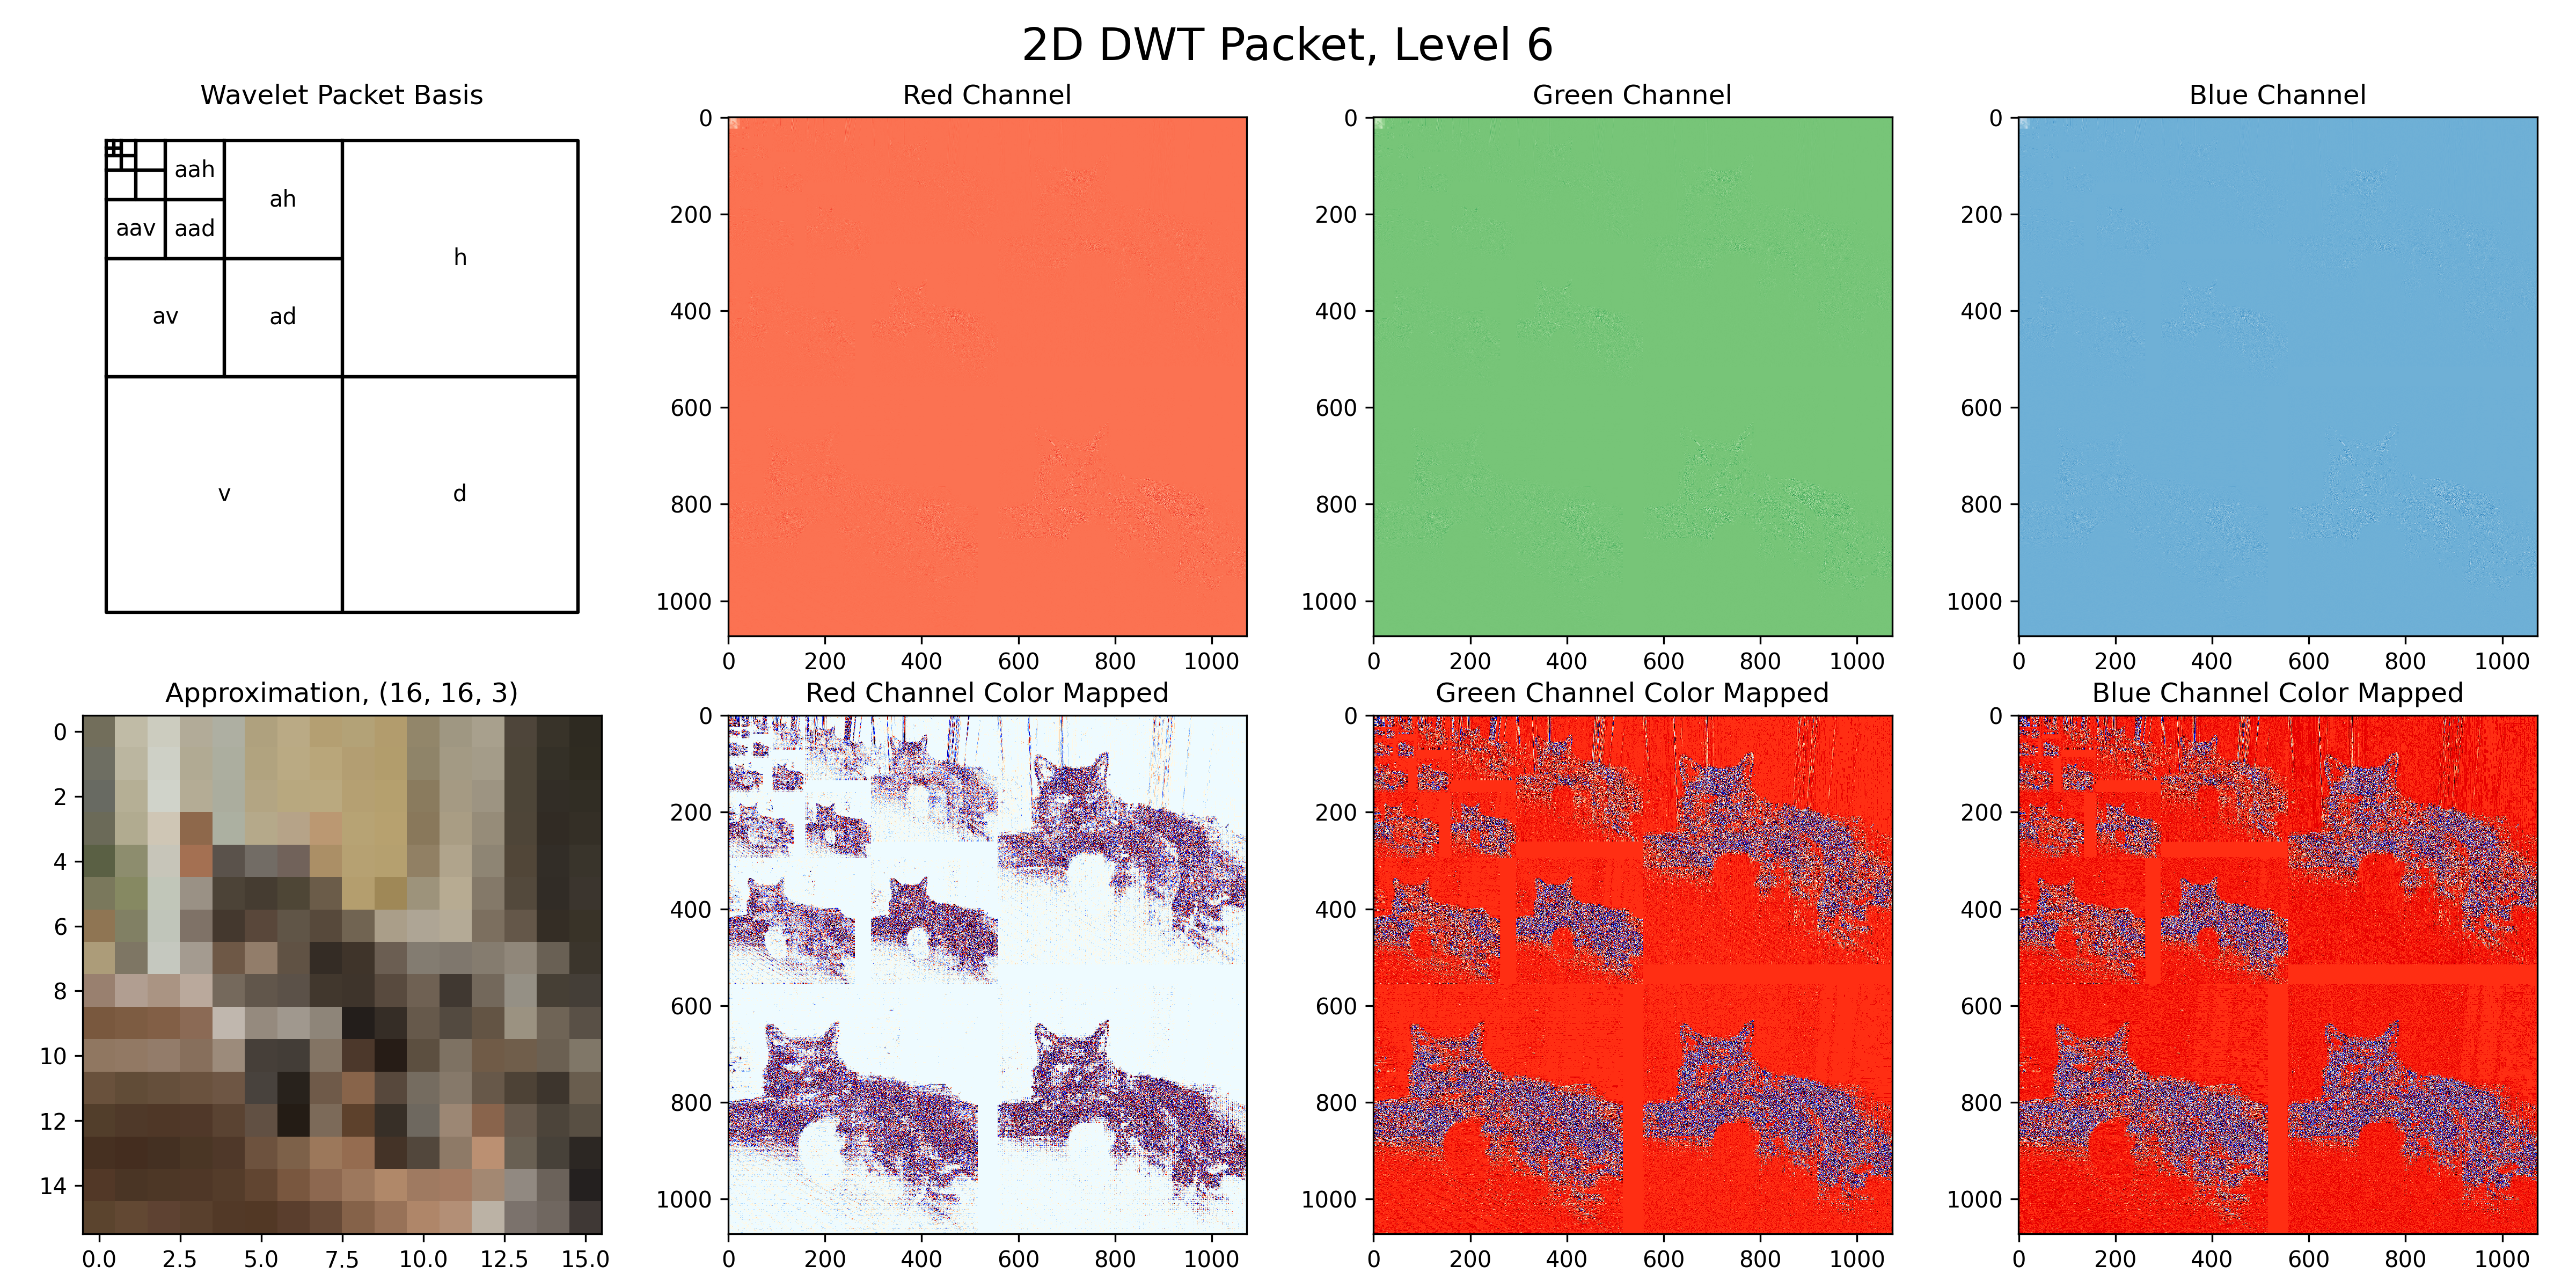
\includegraphics[scale=0.25]{./plots/level_6.png}
	\end{figure}
\end{frame}


\begin{frame}{What's left?}
	There are two \textbf{major} steps left to the JPEG2000 algorithm that
	are outside the scope of this presentation. Quantization and encoding.

	\vspace{1cm}

	This project used the CDF 9/7 wavelet, which is intended to be used
	for lossy compression. Consider applying a pointwise threshold to
	each pixel in the detail coefficients. This is quantization.

	\vspace{0.5cm}

	Encoding is the method through which the quantized coefficients are
	stored in a file. In common practice, the Embedded Block Coding with
	Optimized Truncation (EBCOT) algorithm is used.
	
\end{frame}

\end{document}